\documentclass{article}
\usepackage{graphicx} % Required for inserting images
\usepackage[colorlinks=true, allcolors=blue]{hyperref}
\usepackage[square,numbers]{natbib}
\usepackage{titlesec}
\usepackage{geometry}
 \geometry{
 a4paper,
 total={170mm,257mm},
 left=20mm,
 top=20mm,
 }
\graphicspath{ {./images/} }

\title{Unit 23}
\author{Chris}
\date{}
\bibliographystyle{abbrvnat}

\begin{document}

\section{How cognitive computing can be used to help improve business activities}

\section{Healthcare}
In an article in PubMed said "Cognitive computing, is an evolving technology in healthcare augments the clinical thought process and enable the doctors to make the right diagnosis and preserve the patient's health in good condition."\cite{pubmed}. Healthcare systems can provide care and optimal and cost-effective treatment according to this article.
There are already a number of cognitive platforms in the area of health including
\begin{itemize}
    \item IBM Watson
    \item Microsoft Cortana Intelligence Suite
    \item Google Deepmind
\end{itemize}



\section{Retail}
Cognitive computing in retail is changing everything in business in the same way as other businesses make decisions. Using AI and Machine Learning , businesses are using cognitive to spot patterns to shoppers behaviours and to shift through all the new data that shoppers are bringing in when they are shopping or online.

\section{Education}
According to Gartner, "The global market for AI in education is projected to reach \$6.1 billion by 2025." \cite{emb} and "72\% of educational institutions are investing in AI-driven technologies to enhance learning outcomes".
These make us think that there are huge improvements to using LLMs in eduction 
\begin{itemize}
    \item Personalized learning you can customize learning experiences for each student
    \item Automated tasks like grading
    \item New tools and resources
    \item Real-time feedback and support
\end{itemize} \cite{packtpub}

\section{Finance}
Computers have always been used in finance since they first became popular. Cognitive computing helps fiance people by improving client-facing services. How client-facing can improve with cognitive computer are doing provide innovative financial advisory solutions that make them better for their customers. How future innovations can improve with cognitive computing is by helping the client to understand big data and see what the future holds.
Chatbots specifically can give
\begin{itemize}
    \item Detailed customer analysis
    \item Contextualized customer service
    \item Improved security and identity management by analyzing customer behaviors
\end{itemize} \cite{pulse}

\section{Diagrams}
Diagram of cognitive computer in healthcare \\
\includegraphics[scale=0.5]{Healthcare} \\
Diagram of cognitive computing \\
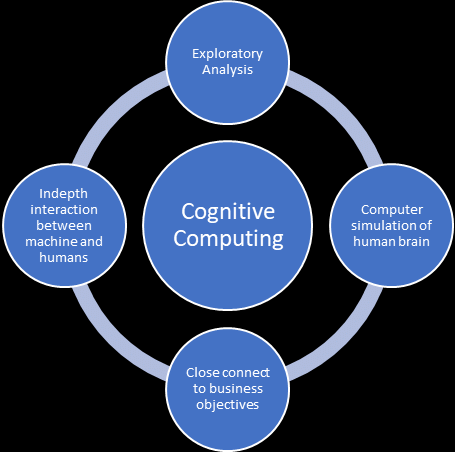
\includegraphics[scale=0.5]{Cognitive} \\

\break
\bibliography{bibliography}

\end{document}
